\documentclass[10pt,letterpaper]{article}
\usepackage[margin=0.75in]{geometry}
\usepackage[T1]{fontenc}\usepackage[utf8]{inputenc}
\usepackage{mathptmx,amsmath,graphicx,caption}
\usepackage[hidelinks]{hyperref}
\hypersetup{pdftitle={EurekaZero: Supplementary Telemetry},pdfauthor={JopeDime Team},pdflang={en-US}}
\renewcommand{\thefigure}{S\arabic{figure}}
\captionsetup{font=small}% captions match the main paper (9pt)
\begin{document}
\section*{EurekaZero: Supplementary Telemetry}
\noindent Candidate movement precedes admission; retention and independent learning
remain separate questions.
\begin{figure}[h]
  \centering
  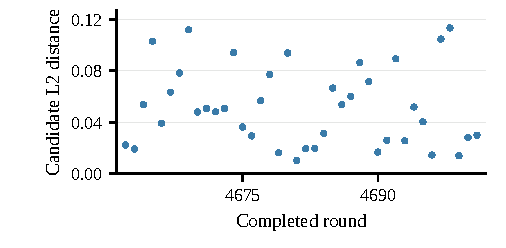
\includegraphics[width=3.375in]{figures/fig_parameter_displacement.pdf}
  \caption{\textbf{Recorded candidate displacement varies across rounds.}
  All 40 complete retained summaries, rounds 4662--4701, captured at
  00:55 UTC on 4 November 2026. Points show logged candidate parameter-space
  L2 displacement; no smoothing or filtering is applied. In the inspected
  loop, it includes warm-restart perturbation and optimization before
  admission. The journal records zero admissions in this window.
  This does not isolate optimizer effects or establish a retained learning
  gain. Scope: the adaptive adapter admission record in the main manuscript.}
  \label{fig:parameter-displacement}
\end{figure}

\begin{figure}[h]
  \centering
  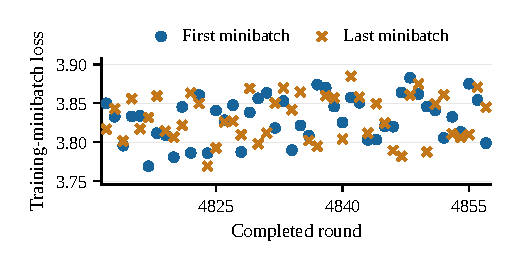
\includegraphics[width=3.375in]{figures/fig_training_minibatch_losses.pdf}
  \caption{\textbf{First and last recorded minibatch losses use different batches.}
  All 46 complete retained summaries, rounds 4812--4857, captured at
  05:53 UTC on 4 November 2026. The 92 points show logged first and last
  training-minibatch objectives, with two optimizer steps per candidate round.
  Batch-order hashes differ within every round; these are not matched
  before/after losses. No smoothing or filtering is applied. The window
  records zero admissions; these losses establish no retained learning gain.
  Scope: the adaptive adapter admission record in the main manuscript.}
  \label{fig:training-minibatch-losses}
\end{figure}
\end{document}
